\documentclass[serif]{beamer}

% ---------------------------------------------------------

\usepackage[utf8]{inputenc}
\usepackage[T1]{fontenc}
\usepackage[english]{babel}

% ---------------------------------------------------------

\usepackage{appendixnumberbeamer}

\setbeamertemplate{navigation symbols}{}

\addtobeamertemplate{footline}{%
	\hspace*{\fill}%
	\llap{%
		\insertframenumber\,/\,\inserttotalframenumber%
		\hspace{5pt}%
	}
	\vskip4pt%
}

\AtBeginSection[]{
	\begin{frame}
		\tableofcontents[currentsection]
	\end{frame}
}

% ---------------------------------------------------------

\usepackage{xcolor}
\usepackage{xspace} % \xspace

\usepackage{graphicx}

\usepackage{stackrel} % \stackrel

\usepackage{fancyvrb} % Verbatim

\usepackage{dashbox} % \dbox

\usepackage{pifont} % \ding

\usepackage{tikz}
\usetikzlibrary{
	decorations.pathreplacing,
	positioning
}

% ---------------------------------------------------------

\usepackage{amsmath} % align*

\usepackage{amssymb} % \mathbb
\usepackage{mathrsfs} % \mathscr
\usepackage{bbm} % \mathbbm
\usepackage{tensor} % \tensor

\usepackage{mathabx} % \ast, \bigast

\usepackage{mathpartir}

\let\oldexists\exists
\let\exists\relax\DeclareMathOperator{\exists}{\oldexists}
\let\oldforall\forall
\let\forall\relax\DeclareMathOperator{\forall}{\oldforall}

\DeclareMathOperator{\lambdaabs}{\lambda}
\DeclareMathOperator{\muabs}{\mu}
\DeclareMathOperator{\nuabs}{\nu}

% ---------------------------------------------------------

\usepackage{listings}
\usepackage{lstcaml}

% ---------------------------------------------------------

\usepackage{overtools}

% ---------------------------------------------------------

\newcommand{\etal}{\textit{et al.}}

\newcommand{\mathhyphen}{{\hbox{-}}}

\newcommand{\eqdef}{\stackrel{\Delta}=}

\newcommand\doubleplus{+\kern-1.3ex+\kern0.8ex}
\newcommand\mdoubleplus{\ensuremath{\mathbin{+\mkern-10mu+}}}

\newcommand{\sref}[1]{\S\ref{#1}}
\newcommand{\fref}[1]{Figure~\ref{#1}}

% ---------------------------------------------------------

\definecolor{cec1d24}{RGB}{236,29,36}
\definecolor{cffffff}{RGB}{255,255,255}

\newcommand{\cmark}{\ding{51}}

\newcommand{\ucmark}{\tikz[y=0.80pt,x=0.80pt,yscale=-0.02,xscale=0.02, inner sep=0pt, outer sep=0pt]%
  {\path[fill=cec1d24,nonzero rule] (635.8833,600.0000) .. controls
    (651.0771,599.6647) and (665.7558,591.6224) .. (673.9783,577.5525) .. controls
    (682.1001,563.3625) and (681.7384,546.6500) .. (674.5074,533.1862) --
    (378.4699,21.6487) .. controls (370.6590,8.7662) and (356.3424,0.0975) ..
    (340.1099,-0.0063) .. controls (323.6499,0.0972) and (309.3362,8.7657) ..
    (301.4862,21.6487) -- (5.4612,533.1862) .. controls (-1.7257,546.6500) and
    (-2.0877,563.3625) .. (5.9903,577.5525) .. controls (14.2570,591.6225) and
    (28.9353,599.6650) .. (44.0853,600.0000) -- (635.8853,600.0000);
    \path[fill=cffffff,nonzero rule] (340.1208,75.7875) -- (71.0683,540.8450) --
    (608.8933,540.8450) -- (340.1058,75.7950);
    \path[fill=black,nonzero rule] (303.5900,225.7800) .. controls
    (280.4500,225.7300) and (276.9200,248.1400) .. (276.8800,250.6200) .. controls
    (276.9200,262.4400) and (285.4000,277.1700) .. (309.1600,279.4100) .. controls
    (309.1600,279.4100) and (313.7700,280.0900) .. (313.6600,283.0900) .. controls
    (313.7700,285.9400) and (313.7800,284.9700) .. (312.3400,286.5300) .. controls
    (310.8500,288.2300) and (298.5500,299.6400) .. (298.3100,302.6600) .. controls
    (296.9800,316.8800) and (300.1800,335.2800) .. (303.0900,345.9400) .. controls
    (303.0900,345.9400) and (306.6000,354.7800) .. (303.8800,361.0000) .. controls
    (301.0600,367.4700) and (289.0000,397.7400) .. (288.0000,399.5600) .. controls
    (285.1300,404.8200) and (284.0000,409.1400) .. (285.8800,415.4100) .. controls
    (284.6600,416.1100) and (264.4700,428.8800) .. (264.4700,428.8800) .. controls
    (264.4700,428.8800) and (261.3500,421.5100) .. (253.5900,419.3800) .. controls
    (245.7000,417.1100) and (239.1800,418.1800) .. (232.7200,405.9100) --
    (226.8800,396.4100) .. controls (226.8800,396.4100) and (225.6700,392.9300) ..
    (219.7500,391.6200) .. controls (213.9300,390.4900) and (206.1000,388.3000) ..
    (202.8100,388.4700) .. controls (198.6100,388.8800) and (195.2200,387.7300) ..
    (189.5900,394.2800) .. controls (185.0800,399.5300) and (112.8800,524.4700) ..
    (112.8800,524.4700) -- (286.4100,524.4700) .. controls (286.4100,524.4700) and
    (290.7100,524.0000) .. (289.5900,519.9700) .. controls (288.2700,516.1900) and
    (267.3800,441.8100) .. (267.3800,441.8100) -- (291.4400,426.7500) .. controls
    (291.4400,426.7500) and (293.3600,429.9900) .. (300.4400,426.7500) .. controls
    (307.3800,423.4800) and (309.9700,421.7500) .. (309.9700,421.7500) .. controls
    (309.9700,421.7500) and (313.9200,421.4900) .. (313.4100,413.0300) .. controls
    (316.1700,411.3100) and (341.9700,395.0600) .. (341.9700,395.0600) .. controls
    (341.9700,395.0600) and (332.8400,417.6000) .. (331.9100,427.5600) .. controls
    (331.2100,437.4600) and (327.6900,504.1200) .. (327.6900,504.1200) .. controls
    (327.6900,504.1200) and (328.1300,509.2200) .. (324.7800,510.2200) .. controls
    (321.2800,511.1700) and (305.7200,515.5000) .. (305.7200,515.5000) .. controls
    (305.7200,515.5000) and (301.3900,516.2100) .. (301.5000,519.7200) .. controls
    (301.3900,523.0400) and (303.0200,524.3400) .. (304.9400,524.4700) .. controls
    (306.9300,524.3400) and (355.7200,524.4700) .. (355.7200,524.4700) .. controls
    (355.7200,524.4700) and (360.7100,525.0000) .. (361.5300,518.4100) .. controls
    (362.3400,511.9900) and (371.5900,445.5000) .. (371.5900,445.5000) .. controls
    (371.5900,445.5000) and (367.5700,444.4500) .. (367.6200,440.5000) .. controls
    (367.5700,436.3200) and (367.5600,433.2000) .. (368.9400,431.5000) .. controls
    (370.1600,429.9500) and (384.8300,413.0400) .. (394.8800,389.5300) .. controls
    (396.4200,386.0300) and (397.5600,389.1300) .. (397.7800,390.0600) .. controls
    (398.2100,390.7500) and (417.2800,442.6600) .. (419.4700,444.7200) .. controls
    (421.8400,446.5600) and (473.3600,488.2300) .. (474.5000,489.0900) .. controls
    (475.6400,489.8600) and (478.9100,492.1100) .. (479.0000,499.3800) .. controls
    (478.9100,506.7600) and (475.9700,512.6300) .. (473.9700,514.9700) .. controls
    (472.0500,517.1900) and (468.8000,520.4500) .. (468.6900,521.8400) .. controls
    (468.8000,523.3800) and (470.2800,524.3400) .. (471.3400,524.4700) .. controls
    (472.5600,524.3400) and (479.2500,524.3400) .. (479.8100,524.4700) .. controls
    (480.5500,524.3400) and (489.3400,525.0100) .. (495.4100,514.1900) .. controls
    (501.7300,503.5300) and (513.1200,484.3400) .. (513.1200,484.3400) .. controls
    (513.1200,484.3400) and (515.5800,480.5600) .. (512.0600,478.2500) .. controls
    (508.4000,476.0100) and (502.7100,474.7100) .. (499.3800,471.1200) .. controls
    (495.8600,467.5500) and (462.9400,429.6400) .. (462.3400,428.8800) .. controls
    (461.9600,428.3400) and (457.7100,423.7600) .. (452.2800,426.2200) .. controls
    (450.7000,424.0900) and (448.8400,421.2200) .. (448.8400,421.2200) .. controls
    (448.8400,421.2200) and (439.4600,364.4600) .. (429.5300,340.4100) .. controls
    (431.8000,339.0000) and (434.8100,336.7200) .. (434.8100,336.7200) .. controls
    (434.8100,336.7200) and (442.7200,343.5500) .. (449.3800,336.4400) .. controls
    (456.0900,329.2300) and (455.6000,329.4100) .. (454.4100,326.1600) .. controls
    (453.3200,322.9000) and (452.8300,321.9100) .. (450.4400,320.5900) .. controls
    (448.2700,319.3000) and (444.5200,315.5500) .. (444.6200,308.9700) .. controls
    (444.5200,302.5400) and (441.7400,284.8000) .. (438.5300,277.2800) .. controls
    (435.5500,269.8300) and (434.5600,261.5500) .. (422.9100,256.4400) .. controls
    (404.4800,248.2100) and (379.8000,243.3100) .. (361.8100,247.9700) .. controls
    (356.8300,249.3000) and (340.8200,261.0500) .. (339.3100,261.9700) .. controls
    (337.8900,262.6800) and (331.6400,265.2600) .. (332.1900,259.8400) .. controls
    (333.4500,247.4700) and (322.7500,225.7300) .. (303.5900,225.7800) --
    cycle(394.8800,275.9700) .. controls (394.8800,275.9700) and
    (408.4700,275.8400) .. (411.5300,276.2200) .. controls (414.3400,276.5000) and
    (416.0300,280.1900) .. (416.0300,280.1900) -- (429.0000,325.8800) --
    (424.2500,328.7800) .. controls (421.5800,323.2700) and (397.9000,287.2600) ..
    (393.0300,280.4700) .. controls (389.9100,276.1000) and (394.8800,275.9700) ..
    (394.8800,275.9700) -- cycle(331.0000,332.8100) .. controls
    (331.5700,332.7900) and (332.2200,332.9700) .. (332.7200,333.2800) .. controls
    (337.8300,336.2000) and (347.5100,344.5400) .. (355.7200,356.0000) .. controls
    (356.7000,357.3200) and (355.7200,361.2800) .. (355.7200,361.2800) --
    (348.5900,376.0600) .. controls (348.5900,376.0600) and (317.8500,395.3700) ..
    (315.5000,396.9100) .. controls (312.9600,398.3000) and (311.5500,396.9300) ..
    (313.9400,393.7500) .. controls (327.6400,375.1200) and (332.7200,353.0000) ..
    (329.5300,335.1200) .. controls (329.2600,333.4800) and (330.0500,332.8500) ..
    (331.0000,332.8100) -- cycle;}}

% ---------------------------------------------------------

\newcommand{\OCaml}{\textsc{OCaml}\xspace}
\newcommand{\Coq}{\textsc{Coq}\xspace}
\newcommand{\Iris}{\textsc{Iris}\xspace}
\newcommand{\C}{\textsc{C}\xspace}
\newcommand{\Cpp}{\textsc{C}\texttt{++}\xspace}
\newcommand{\Rust}{\textsc{Rust}\xspace}
\newcommand{\Go}{\textsc{Go}\xspace}

% ---------------------------------------------------------

\newcommand{\weakestpre}[2]{%
	\mathrm{WP}\ #1\ \left\lbrace\, #2 \,\right\rbrace%
}

\newcommand{\triple}[3]{%
	\left\lbrace\, #1 \,\right\rbrace\ %
	#2\ %
	\left\lbrace\, #3 \,\right\rbrace%
}
\newcommand{\triplePretty}[3]{%
	\begin{array}{c}
			\left\lbrace\, #1 \,\right\rbrace
		\\ \hline
			#2
		\\ \hline
			\left\lbrace\, #3 \,\right\rbrace
	\end{array}
}
\newcommand{\atriple}[6]{%
	\left\langle\, \forall #1 .\ #2 \,\right\rangle\ %
	#3\ %
	\left\langle\, \exists #4 .\ #5 .\ #6 \,\right\rangle%
}
\newcommand{\atriplePretty}[6]{%
	\begin{array}{c}
			\left\langle\, \forall #1 .\ #2 \,\right\rangle
		\\ \hline
			#3
		\\ \hline
			\left\langle\, \exists #4 .\ #5 .\ #6 \,\right\rangle
	\end{array}
}
\newcommand{\atripleExt}[9]{%
	\left\lbrace\, #1 \,\right\rbrace\ %
	\left\langle\, \forall #2 .\ #3 \,\right\rangle\ %
	#4,\ #5\ %
	\left\langle\, \exists #6 .\ #7 \,\right\rangle\ %
	\left\lbrace\, #8 .\ #9 \,\right\rbrace%
}
\newcommand{\atripleExtPretty}[9]{%
	\begin{array}{c}
			\left\lbrace\, #1 \,\right\rbrace
		\\ \hline
			\left\langle\, \forall #2 .\ #3 \,\right\rangle
		\\ \hline
			#4,\ #5
		\\ \hline
			\left\langle\, \exists #6 .\ #7 \,\right\rangle
		\\ \hline
			\left\lbrace\, #8 .\ #9 \,\right\rbrace
	\end{array}
}

% ---------------------------------------------------------

\newcommand{\term}[1]{\texttt{#1}}
\newcommand{\nterm}[1]{\mathrm{#1}}

\newcommand{\exprUnit}{\term{(}\term{)}}
\newcommand{\exprRef}[1]{\term{ref}\ #1}
\newcommand{\exprSeq}[2]{#1\,\term{;}\,#2}
\newcommand{\exprIf}[3]{\term{if}\ #1\ \term{then}\ #2\ \term{else}\ #3}
\newcommand{\exprLoad}[1]{!\,#1}
\newcommand{\exprStore}[2]{#1\leftarrow#2}
\newcommand{\exprCall}[2]{#1\ #2}
\newcommand{\exprNone}{\term{NONE}}
\newcommand{\exprSome}[1]{\term{SOME}\ #1}

% ---------------------------------------------------------

\newcommand{\iEmpty}{\emptyset}
\newcommand{\iTrue}{\mathrm{True}}
\newcommand{\iFalse}{\mathrm{False}}
\newcommand{\iSep}{\ast}
\newcommand{\iBigsep}{\bigast}
\newcommand{\iSepimp}{\mathrel{-\mkern-6mu\iSep}}
\newcommand{\iBupd}{|\!\!\!\Rrightarrow}
\newcommand{\iPers}{\square}
\newcommand{\iAuth}[1]{\bullet\,#1}
\newcommand{\iFrag}[1]{\circ\,#1}
\newcommand{\iGhost}[2]{\dbox{\strut\ensuremath{#2}}^{#1}}
\newcommand{\iInv}[2]{\boxed{\strut\ensuremath{#2}}^{#1}}


% ---------------------------------------------------------

\title{
	Verification of Chase-Lev work-stealing deque \\
	(work in progress)
}
\author{
	\underline{Clément Allain} \\
	François Pottier
}
\institute{
	Inria Paris
}

% ---------------------------------------------------------
% ---------------------------------------------------------

\begin{document}

% ---------------------------------------------------------

\begin{frame}
\titlepage
\end{frame}

% ---------------------------------------------------------

\begin{frame}[fragile]{Verification of a scheduler}
%\begin{itemize}
%	\item domainslib (\OCaml~5)
%	\item Taskflow (C++)
%\end{itemize}
%\vfill
\begin{Verbatim}[commandchars=\\\{\}]
let rec fib pool n =
  if n < 2 then 1 else
  let r1 = \textcolor{blue}{async} pool (fun () -> fib_par (n - 1)) in
  let r2 = \textcolor{blue}{async} pool (fun () -> fib_par (n - 2)) in
  \textcolor{blue}{await} pool r1 + \textcolor{blue}{await} pool r2
\end{Verbatim}
\end{frame}
\begin{frame}{Work-stealing}
\centering
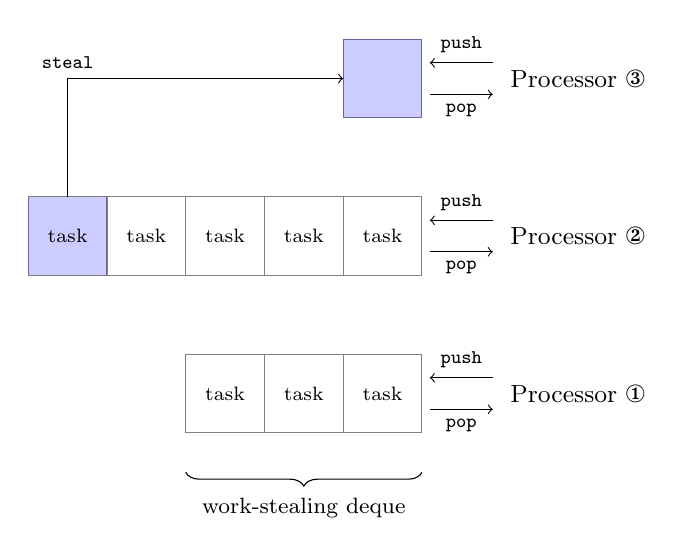
\begin{tikzpicture}
	\def\sep{1}
	\def\hsep{0.1}
	\def\vsep{0.3}
	\def\lenI{3}
	\def\lenxI{0}
	\def\lenII{4}
	\def\lenxII{1}
	\def\lenIII{0}
	\def\lenxIII{1}
	
	\node[right] at (1, 0.5) {\small Processor \ding{172}} ;
	\draw[step=1cm, gray] (0, 0) grid ++(-\lenI, 1) ;
	\draw[step=1cm, gray] (-\lenI, 0) grid ++(-\lenxI, 1) ;
	\fill[blue, opacity=0.2] (-\lenI, 0) rectangle ++(-\lenxI, 1) ;
	\draw[decorate, decoration={brace, amplitude=5pt}] (0, -0.5) -- ++(-\lenI, 0) node [midway, below, yshift=-2mm] {\footnotesize work-stealing deque} ;
	\draw[->] (\hsep, \vsep) -- ++(1 - 2 * \hsep, 0) node[midway, below] {\scriptsize\texttt{pop}} ;
	\draw[->] (1 - \hsep, 1 - \vsep) -- ++(2 * \hsep - 1, 0) node[midway, above] {\scriptsize\texttt{push}} ;
	\foreach \x in {1, ..., \lenI} {
		\node at (0.5 - \x, 0.5) {\scriptsize task} ;
	}
	
	\node[right] at (1, \sep + 1.5) {\small Processor \ding{173}} ;
	\draw[step=1cm, gray] (0, \sep + 1) grid ++(-\lenII, 1) ;
	\draw[step=1cm, gray] (-\lenII, \sep + 1) grid ++(-\lenxII, 1) ;
	\fill[blue, opacity=0.2] (-\lenII, \sep + 1) rectangle ++(-\lenxII, 1) ;
	\draw[->] (\hsep, \sep + 1 + \vsep) -- ++(1 - 2 * \hsep, 0) node[midway, below] {\scriptsize\texttt{pop}} ;
	\draw[->] (1 - \hsep, \sep + 2 - \vsep) -- ++(2 * \hsep - 1, 0) node[midway, above] {\scriptsize\texttt{push}} ;
	\foreach \x in {1, ..., \lenII} {
		\node at (0.5 - \x, \sep + 1.5) {\scriptsize task} ;
	}
	\node at (0.5 - \lenII - \lenxII, \sep + 1.5) {\scriptsize task} ;
	
	\node[right] at (1, 2 * \sep + 2.5) {\small Processor \ding{174}} ;
	\draw[step=1cm, gray] (0, 2 * \sep + 2) grid ++(-\lenIII, 1) ;
	\draw[step=1cm, gray] (-\lenIII, 2 * \sep + 2) grid ++(-\lenxIII, 1) ;
	\fill[blue, opacity=0.2] (-\lenIII, 2 * \sep + 2) rectangle ++(-\lenxIII, 1) ;
	\draw[->] (\hsep, 2 * \sep + 2 + \vsep) -- ++(1 - 2 * \hsep, 0) node[midway, below] {\scriptsize\texttt{pop}} ;
	\draw[->] (1 - \hsep, 2 * \sep + 3 - \vsep) -- ++(2 * \hsep - 1, 0) node[midway, above] {\scriptsize\texttt{push}} ;
	
	\draw[->, to path={|- node[above] {\scriptsize\texttt{steal}} (\tikztotarget)}] (0.5 - \lenII - \lenxII, \sep + 2) to (- \lenIII - \lenxIII, 2 * \sep + 2.5) ;
\end{tikzpicture}
\end{frame}

% ---------------------------------------------------------

\begin{frame}{Chase-Lev work-stealing deque}
\begin{enumerate}
	\item
		\textit{The Implementation of the Cilk-5 Multithreaded Language}. \\
		Frigo, Leiserson \& Randall (1998).
		\begin{itemize}
			\item lock
		\end{itemize}
	\item
		\textit{Thread Scheduling for Multiprogrammed Multiprocessors}. \\
		Arora, Blumofe \& Plaxton (1998).
		\begin{itemize}
			\item non-blocking
			\item one fixed size array, potential overflow
		\end{itemize}
	\item
		\textit{A dynamic-sized nonblocking work stealing deque}. \\
		Hendler, Lev, Moir \& Shavit (2004).
		\begin{itemize}
			\item non-blocking
			\item list of small arrays, no overflow
		\end{itemize}
	\item
		\underline{\textit{Dynamic circular work-stealing deque}}. \\
		Chase \& Lev (2005).
		\begin{itemize}
			\item non-blocking
			\item circular arrays, no overflow
		\end{itemize}
\end{enumerate}
\end{frame}
\begin{frame}{Why is it interesting?}
\begin{itemize}
	\item demonstration of Iris on a (simplified) real-life concurrent data structure
	\item rich ghost state to enforce a subtle protocol
		\begin{itemize}
			\item logical state $\neq$ physical state
			\item external future-dependent linearization point
		\end{itemize}
	\item use of prophecy variables (with memory)
\end{itemize}
\end{frame}

\begin{frame}{The rest of this talk}
\begin{itemize}
	\item specification using logically atomic triples
	\item rough idea of how the data structure works
	\item why we need prophecy variables (with memory)
\end{itemize}
\end{frame}
\section{Specification}

\begin{frame}{Specification --- \texttt{chaselev\_make}}
\small
\centering
\[
	\triplePretty{
		\iTrue
	}{
		\texttt{chaselev\_make}\ \exprUnit
	}{
		\lambda\ t .\ 
		\tikz[baseline, remember picture]{\node[anchor=base] (inv_1) {${
			\textcolor{blue}{\mathrm{chaselev \mathhyphen inv}\ t\ \iota}
		}$}} \iSep
		\tikz[baseline, remember picture]{\node[anchor=base] (model_1) {${
			\textcolor{red}{\mathrm{chaselev \mathhyphen model}\ t\ []}
		}$}} \iSep
		\tikz[baseline, remember picture]{\node[anchor=base] (owner_1) {${
			\textcolor{teal}{\mathrm{chaselev \mathhyphen owner}\ t}
		}$}}
	}
\]
\vfill
\only<2>{
	\tikz[remember picture] \node[align=left] (inv_2) {
		$t$ is an instance of Chase-Lev deque. \\
		Enforces a protocol (using an Iris invariant).
	} ;
	\begin{tikzpicture}[remember picture, overlay]
		\path[draw=blue, thick, ->] (inv_2.north) to [out=100, in=-100] (inv_1.south) ;
	\end{tikzpicture}
}
\only<3>{
	\tikz[remember picture] \node[align=left] (model_2) {
		Asserts the list of values that $t$ logically contains.
	} ;
	\begin{tikzpicture}[remember picture, overlay]
		\path[draw=red, thick, ->] (model_2.north) to [out=100, in=-100] (model_1.south) ;
	\end{tikzpicture}
}
\only<4>{
	\tikz[remember picture] \node[align=left] (owner_2) {
		Gives the owner exclusive access to his end of $t$.
	} ;
	\begin{tikzpicture}[remember picture, overlay]
		\path[draw=teal, thick, ->] (owner_2.north) to [out=100, in=-100] (owner_1.south) ;
	\end{tikzpicture}
}
\end{frame}

% ---------------------------------------------------------

\begin{frame}{Specification --- \texttt{chaselev\_push}}
\centering
\[
	\atripleExtPretty{
		\tikz[baseline, remember picture]{\node[anchor=base] (inv_1) {${
			\textcolor{blue}{\mathrm{chaselev \mathhyphen inv}\ t\ \iota}
		}$}} \iSep
		\tikz[baseline, remember picture]{\node[anchor=base] (owner_1) {${
			\textcolor{red}{\mathrm{chaselev \mathhyphen owner}\ t}
		}$}}
	}{
		\mathit{vs}
	}{
		\tikz[baseline, remember picture]{\node[anchor=base] (model_1) {${
			\textcolor{teal}{\mathrm{chaselev \mathhyphen model}\ t\ \mathit{vs}}
		}$}}
	}{
		\texttt{chaselev\_push}\ t\ v
	}{
		\uparrow\iota
	}{
	}{
		\tikz[baseline, remember picture]{\node[anchor=base] (model_2) {${
			\textcolor{teal}{\mathrm{chaselev \mathhyphen model}\ t\ (\mathit{vs} \mdoubleplus [v])}
		}$}}
	}{
		\exprUnit
	}{
		\tikz[baseline, remember picture]{\node[anchor=base] (owner_2) {${
			\textcolor{red}{\mathrm{chaselev \mathhyphen owner}\ t}
		}$}}
	}
\]
\begin{overbox}<2>
	\small
	\centering
	Specification of a concurrent operation ($\simeq$ transaction):
	
	standard triple + logically atomic triple
	
	\[
		\atripleExtPretty{
			\textcolor{red}{P}
		}{
			\textcolor{purple}{\overline{x}}
		}{
			\textcolor{teal}{P_\mathrm{lin}}
		}{
			e
		}{
			\mathcal{E}
		}{
			\textcolor{purple}{\overline{y}}
		}{
			\textcolor{teal}{Q_\mathrm{lin}}
		}{
			res
		}{
			\textcolor{red}{Q}
		}
	\]
	\begin{align*}
			\textcolor{red}{P}
			&:
			\text{private precondition}
		\\
			\textcolor{red}{Q}
			&:
			\text{private postcondition}
		\\
			\textcolor{teal}{P_\mathrm{lin}}
			&:
			\text{public precondition}
		\\
			\textcolor{teal}{Q_\mathrm{lin}}
			&:
			\text{public postcondition}
	\end{align*}
\end{overbox}
\begin{overbox}<3>
	For a concurrent data structure:
	
	\[
		\atripleExtPretty{
			\textcolor{blue}{\mathrm{??? \mathhyphen inv} \cdots} \iSep
			\textcolor{red}{P}
		}{
			\textcolor{purple}{\overline{x}}
		}{
			\textcolor{teal}{\mathrm{??? \mathhyphen model} \cdots}
		}{
			e
		}{
			\mathcal{E}
		}{
			\textcolor{purple}{\overline{y}}
		}{
			\textcolor{teal}{\mathrm{??? \mathhyphen model} \cdots}
		}{
			res
		}{
			\textcolor{red}{Q}
		}
	\]
\end{overbox}
\vfill
\only<4>{
	\tikz[remember picture] \node[align=left] (inv_2) {
		$t$ is an instance of Chase-Lev deque.
	} ;
	\begin{tikzpicture}[remember picture, overlay]
		\path[draw=blue, thick, ->] (inv_2.north) to [out=100, in=-100] (inv_1.south) ;
	\end{tikzpicture}
}
\only<5>{
	\tikz[remember picture] \node[align=left] (owner_3) {
		This operation is reserved to the owner of $t$.
	} ;
	\begin{tikzpicture}[remember picture, overlay]
		\path[draw=red, thick, ->] (owner_3.north) to [out=100, in=-100] (owner_1.south) ;
		\path[draw=red, thick, ->] (owner_3.north) to [out=100, in=-100] ([xshift=5mm]owner_2.south) ;
	\end{tikzpicture}
}
\only<6>{
	\tikz[remember picture] \node[align=left] (model_3) {
		$v$ is atomically pushed at the owner's end of $t$.
	} ;
	\begin{tikzpicture}[remember picture, overlay]
		\path[draw=teal, thick, ->] (model_3.north) to [out=100, in=-100] (model_1.south) ;
		\path[draw=teal, thick, ->] (model_3.north) to [out=100, in=-100] ([xshift=1cm]model_2.south) ;
	\end{tikzpicture}
}
\end{frame}

% ---------------------------------------------------------

\begin{frame}{Specification --- \texttt{chaselev\_pop}}
\footnotesize
\centering
\[
	\atripleExtPretty{
		\tikz[baseline, remember picture]{\node[anchor=base] (inv_1) {${
			\textcolor{blue}{\mathrm{chaselev \mathhyphen inv}\ t\ \iota}
		}$}} \iSep
		\tikz[baseline, remember picture]{\node[anchor=base] (owner_1) {${
			\textcolor{red}{\mathrm{chaselev \mathhyphen owner}\ t}
		}$}}
	}{
		\mathit{vs}
	}{
		\tikz[baseline, remember picture]{\node[anchor=base] (model_1) {${
			\textcolor{teal}{\mathrm{chaselev \mathhyphen model}\ t\ \mathit{vs}}
		}$}}
	}{
		\texttt{chaselev\_pop}\ t
	}{
		\uparrow\iota
	}{
		o
	}{
		\tikz[baseline, remember picture]{\node[anchor=base] (model_2) {${
			\textcolor{teal}{
				\bigvee\left[\begin{array}{l}
						\mathit{vs} = [] \iSep
						o = \exprNone \iSep
						\textcolor{teal}{\mathrm{chaselev \mathhyphen model}\ t\ []}
					\\
						\exists v, \mathit{vs'} .\ 
						\mathit{vs} = \mathit{vs'} \mdoubleplus [v] \iSep
						o = \exprSome{v} \iSep
						\textcolor{teal}{\mathrm{chaselev \mathhyphen model}\ t\ \mathit{vs'}}
				\end{array}\right]
			}
		}$}}
	}{
		o
	}{
		\tikz[baseline, remember picture]{\node[anchor=base] (owner_2) {${
			\textcolor{red}{\mathrm{chaselev \mathhyphen owner}\ t}
		}$}}
	}
\]
\vfill
\only<2>{
	\tikz[remember picture] \node[align=left] (inv_2) {
		$t$ is an instance of Chase-Lev deque.
	} ;
	\begin{tikzpicture}[remember picture, overlay]
		\path[draw=blue, thick, ->] (inv_2.north) to [out=100, in=-100] (inv_1.south) ;
	\end{tikzpicture}
}
\only<3>{
	\tikz[remember picture] \node[align=left] (owner_3) {
		This operation is reserved to the owner of $t$.
	} ;
	\begin{tikzpicture}[remember picture, overlay]
		\path[draw=red, thick, ->] (owner_3.north) to [out=100, in=-100] (owner_1.south) ;
		\path[draw=red, thick, ->] (owner_3.north) to [out=100, in=-100] ([xshift=5mm]owner_2.south) ;
	\end{tikzpicture}
}
\only<4>{
	\tikz[remember picture] \node[align=left] (model_3) {
		Either 1) $t$ is seen empty \\
		or 2) some value $v$ is atomically popped at the owner's end of $t$.
	} ;
	\begin{tikzpicture}[remember picture, overlay]
		\path[draw=teal, thick, ->] (model_3.north) to [out=100, in=-100] (model_1.south) ;
		\path[draw=teal, thick, ->] (model_3.north) to [out=100, in=-100] ([xshift=1cm]model_2.south) ;
	\end{tikzpicture}
}
\end{frame}

% ---------------------------------------------------------

\begin{frame}{Specification --- \texttt{chaselev\_steal}}
\footnotesize
\centering
\[
	\atripleExtPretty{
		\tikz[baseline, remember picture]{\node[anchor=base] (inv_1) {${
			\textcolor{blue}{\mathrm{chaselev \mathhyphen inv}\ t\ \iota}
		}$}}
	}{
		\mathit{vs}
	}{
		\tikz[baseline, remember picture]{\node[anchor=base] (model_1) {${
			\textcolor{teal}{\mathrm{chaselev \mathhyphen model}\ t\ \mathit{vs}}
		}$}}
	}{
		\texttt{chaselev\_steal}\ t
	}{
		\uparrow\iota
	}{
		o
	}{
		\tikz[baseline, remember picture]{\node[anchor=base] (model_2) {${
			\textcolor{teal}{
				\bigvee\left[\begin{array}{l}
						\mathit{vs} = [] \iSep
						o = \exprNone \iSep
						\mathrm{chaselev \mathhyphen model}\ t\ []
					\\
						\exists v, \mathit{vs'} .\ 
						\mathit{vs} = v :: \mathit{vs'} \iSep
						o = \exprSome{v} \iSep
						\mathrm{chaselev \mathhyphen model}\ t\ \mathit{vs'}
				\end{array}\right]
			}
		}$}}
	}{
		o
	}{
		\iTrue
	}
\]
\vfill
\only<2>{
	\tikz[remember picture] \node[align=left] (inv_2) {
		$t$ is an instance of Chase-Lev deque.
	} ;
	\begin{tikzpicture}[remember picture, overlay]
		\path[draw=blue, thick, ->] (inv_2.north) to [out=100, in=-100] (inv_1.south) ;
	\end{tikzpicture}
}
\only<3>{
	\tikz[remember picture] \node[align=left] (model_3) {
		Either 1) $t$ is seen empty \\
		or 2) some value $v$ is atomically popped at the thieves' end of $t$.
	} ;
	\begin{tikzpicture}[remember picture, overlay]
		\path[draw=teal, thick, ->] (model_3.north) to [out=100, in=-100] (model_1.south) ;
		\path[draw=teal, thick, ->] (model_3.north) to [out=100, in=-100] ([xshift=1cm]model_2.south) ;
	\end{tikzpicture}
}
\end{frame}
\section{Physical state}

\begin{frame}{Physical state}
\centering
\hspace{-1cm}
\begin{tikzpicture}[scale=1.15]
	\def\hist{2}
	\def\histx{1}
	\def\model{3}
	\def\priv{2.8}

	\only<1->{
		\draw[step=1cm, gray] (0, 0) grid ++(\hist + \model + \priv, 1) ;
		\draw[decorate, decoration={brace, amplitude=5pt}] (-0.2, 0) -- ++(0, 1) node [midway, xshift=-7mm] {data} ;
	}

	\only<2->{
		\draw[very thick] (\hist, 0) -- ++(0, 1) node[label=above:front] {} ;
	}

	\only<4->{
		\draw[very thick] (\hist + \model, 0) -- ++(0, 1) node[label=above:back] {} ;
	}

	\only<5->{
		\fill[red, opacity=0.2] (\hist + \model, 0) rectangle ++(\priv, 1) ;
		\draw[decorate, decoration={brace, amplitude=5pt}] (\hist + \model + \priv, -0.2) -- ++(- \priv, 0) node [midway, yshift=-5mm] {priv} ;
	}

	\only<6->{
		\fill[green, opacity=0.2] (\hist, 0) rectangle ++(\model, 1) ;
		\draw[decorate, decoration={brace, amplitude=5pt}] (\hist + \model, -0.2) -- ++(- \model, 0) node [midway, yshift=-5mm] {model} ;
	}
	\only<7->{
		\fill[blue, opacity=0.2] (0, 0) rectangle ++(\hist, 1) ;
		\draw[decorate, decoration={brace, amplitude=5pt}] (\hist, -0.2) -- ++(- \hist, 0) node [midway, yshift=-5mm] {hist} ;
	}

	\only<9->{
		\fill[blue, opacity=0.2] (\hist, 0) rectangle ++(\histx, 1) ;
		\draw[decorate, decoration={brace, amplitude=5pt}] (\hist + \histx, - 1) -- ++(- \hist - \histx, 0) node [midway, yshift=-5mm] {hist\textsubscript{+}} ;
	}

	\only<2->{
		\draw[thick, ->, blue] (\hist, 0.5) -- ++(1, 0) node[midway, below] {\footnotesize\texttt{steal}} ;
	}
	
	\only<4->{
		\draw[thick, ->, teal] (\hist + \model, 0.5) -- ++(- 1, 0) node[midway, below] {\footnotesize\texttt{pop}} ;
		\draw[thick, ->, red] (\hist + \model, 0.5) -- ++(1, 0) node[midway, below] {\footnotesize\texttt{push}} ;
	}
\end{tikzpicture}
\vfill
\begin{itemize}
	\item[data:]<1-> infinite array storing all values
	\item[front:]<2-> \emph{monotone} index for thieves' end
	\item[back:]<4-> index for owner's end
\end{itemize}
\begin{itemize}
	\item[priv:]<5-> list of private values (controlled by owner)
	\item[model:]<6-> list of contained values
	\item[hist:]<7-> \emph{monotone} list of history values
	\item[hist\textsubscript{+}:]<9-> \emph{monotone} list of extended history values
\end{itemize}
\begin{overbox}<3>
	\begin{mathpar}
		\inferrule*[lab=ChaselevFrontLbGet]
			{
				\iGhost{\gamma\mathrm{.front}}{\iAuth{\textcolor{blue}{front}}}
			}{
				\iGhost{\gamma\mathrm{.front}}{\iFrag{\textcolor{blue}{front}}}
			}
		\and
		\inferrule*[lab=ChaselevFrontValid]
			{
				\iGhost{\gamma\mathrm{.front}}{\iAuth{\textcolor{blue}{front_1}}}
			\and
				\iGhost{\gamma\mathrm{.front}}{\iFrag{\textcolor{red}{front_2}}}
			}{
				\textcolor{red}{front_2} \leq \textcolor{blue}{front_1}
			}
		\and
		\inferrule*[lab=ChaselevFrontUpdate]
			{
				\textcolor{blue}{front} \leq \textcolor{red}{front'}
			\and
				\iGhost{\gamma\mathrm{.front}}{\iAuth{\textcolor{blue}{front}}}
			}{
				\iGhost{\gamma\mathrm{.front}}{\iAuth{\textcolor{red}{front'}}}
			}
	\end{mathpar}
\end{overbox}
\begin{overbox}<8>
	\begin{mathpar}
		\inferrule*[lab=ChaselevHistLbGet]
			{
				\iGhost{\gamma\mathrm{.hist}}{\iAuth{\textcolor{blue}{hist}}}
			}{
				\iGhost{\gamma\mathrm{.hist}}{\iFrag{\textcolor{blue}{hist}}}
			}
		\and
		\inferrule*[lab=ChaselevHistValid]
			{
				\iGhost{\gamma\mathrm{.hist}}{\iAuth{\textcolor{blue}{hist_1}}}
			\and
				\iGhost{\gamma\mathrm{.hist}}{\iFrag{\textcolor{red}{hist_2}}}
			}{
				\textcolor{red}{hist_2} \sqsubseteq_\mathrm{prefix} \textcolor{blue}{hist_1}
			}
		\and
		\inferrule*[lab=ChaselevHistUpdate]
			{
				\iGhost{\gamma\mathrm{.hist}}{\iAuth{\textcolor{blue}{hist}}}
			}{
				\iGhost{\gamma\mathrm{.hist}}{\iAuth{(\textcolor{blue}{hist} \mdoubleplus [v])}}
			}
	\end{mathpar}
\end{overbox}
\end{frame}

\begin{frame}{Logical state}
\centering
\begin{tikzpicture}
	\def\width{4cm}
	\def\height{2cm}

	\only<1->{
		\node[align=center] (s1) {
			\ding{172} empty \\
			\begin{tikzpicture}[scale=0.5]
				\def\hist{2}
				\def\priv{2.8}

				\draw[step=1cm, gray] (0, 0) grid (\hist + \priv, 1) ;

				\fill[blue, opacity=0.2] (0, 0) rectangle (\hist, 1) ;
				\draw[very thick] (\hist, 1) -- ++(0, - 1) node[yshift=2mm, label=below:{\tiny front = back}] {} ;
				\fill[red, opacity=0.2] (\hist, 0) rectangle ++(\priv, 1) ;
			\end{tikzpicture}
	   } ;

	   \node[align=center] (s2) [right=\width of s1] {
	   		\ding{173} non-empty \\
			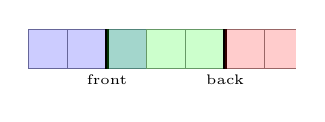
\begin{tikzpicture}[scale=0.5]
				\def\hist{2}
				\def\histx{1}
				\def\model{3}
				\def\priv{1.8}

				\draw[step=1cm, gray] (0, 0) grid (\hist + \model + \priv, 1) ;

				\fill[blue, opacity=0.2] (0, 0) rectangle (\hist + \histx, 1) ;
				\draw[very thick] (\hist, 1) -- ++(0, - 1) node[yshift=2mm, label=below:{\tiny front}] {} ;
				\fill[green, opacity=0.2] (\hist, 0) rectangle ++(\model, 1) ;
				\draw[very thick] (\hist + \model, 1) -- ++(0, - 1) node[yshift=2mm, label=below:{\tiny back}] {} ;
				\fill[red, opacity=0.2] (\hist + \model, 0) rectangle ++(\priv, 1) ;
			\end{tikzpicture}
	   } ;
   }

   \only<3->{
	   \node[align=center] (s3) [below=\height of s2] {
	   		\ding{174} emptyish \\
			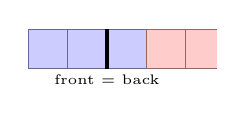
\begin{tikzpicture}[scale=0.5]
				\def\hist{2}
				\def\histx{1}
				\def\priv{2.8}

				\draw[step=1cm, gray] (0, 0) grid (\hist + \priv, 1) ;

				\fill[blue, opacity=0.2] (0, 0) rectangle (\hist + \histx, 1) ;
				\draw[very thick] (\hist, 1) -- ++(0, - 1) node[yshift=2mm, label=below:{\tiny front = back}] {} ;
				\fill[red, opacity=0.2] (\hist + \histx, 0) rectangle ++(\priv - \histx, 1) ;
			\end{tikzpicture}
	   } ;
	   \node[align=center] (s4) [below=\height of s1] {
	   	\ding{175} super empty \\
			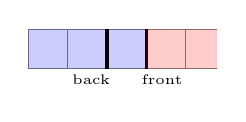
\begin{tikzpicture}[scale=0.5]
				\def\hist{2}
				\def\histx{1}
				\def\priv{2.8}

				\draw[step=1cm, gray] (0, 0) grid (\hist + \priv, 1) ;

				\fill[blue, opacity=0.2] (0, 0) rectangle (\hist + \histx, 1) ;
				\draw[very thick] (\hist, 1) -- ++(0, - 1) node[xshift=-2mm, yshift=2mm, label=below:{\tiny back}] {} ;
				\draw[very thick] (\hist + \histx, 1) -- ++(0, - 1) node[xshift=2mm, yshift=2mm, label=below:{\tiny front}] {} ;
				\fill[red, opacity=0.2] (\hist + \histx, 0) rectangle ++(\priv - \histx, 1) ;
			\end{tikzpicture}
	   } ;
   }

   \only<2->{
	   \draw[thick, ->] (s1) to[bend left] node[above] {\texttt{push}} (s2) ;
	   \draw[thick, ->] (s2) to[bend left] node[below] {\texttt{steal}} (s1) ;
	   \draw[thick, ->] (s2) to[looseness=3, out=135, in=45] node[above] {\texttt{push}, \texttt{pop}, \texttt{steal}} (s2) ;
   }
   \only<4->{
	   \draw[thick, ->] (s2) to[bend left] node[right] {\texttt{pop}} (s3) ;
	   \draw[thick, dotted, ->] (s3) to[bend left] node[below] {\texttt{pop}, \texttt{steal}} (s4) ;
	   \draw[thick, dotted, ->] (s4) to[bend left] node[left] {\texttt{pop}} (s1) ;
   }
   \only<5->{
   		\draw[thick, ->] (s1) to[bend left] node[right] {\texttt{pop}} (s4) ;
   		\draw[thick, dotted, ->] ([xshift=2mm]s1.south) to[bend left] ([xshift=2mm]s4.north) ;
   }

   \only<2-3>{
	   \matrix [below right, nodes={font=\tiny}] at (current bounding box.south west) {
	   		\draw[thick, ->] (0, 0) -- (1em, 0) node[right] {linearization} ; \\
	   } ;
   }
   \only<4->{
	   \matrix [right, nodes={font=\tiny}] at (current bounding box.south west) {
	   		\draw[thick, ->] (0, 0) -- (1em, 0) node[right] {linearization} ; \\
	   		\draw[thick, dotted, ->] (0, 0) -- (1em, 0) node[right] {stabilization} ; \\
	   } ;
   }
\end{tikzpicture}
\end{frame}

\begin{frame}{Prophecy variable}
\[
	\begin{array}{c}
			\triple{
				\iTrue
			}{
				\texttt{NewProph}
			}{
				\lambda\ p \cdot
				\exists prophs \cdot
				\textcolor{blue}{\mathrm{proph}\ p\ prophs}
			}
		\\\\\\
			\inferrule*
				{
					\mathrm{atomic}\ e
				\\\\
					\textcolor{blue}{\mathrm{proph}\ p\ prophs}
				\\\\
					\weakestpre{
						e
					}{
						\begin{array}{l}
								\lambda w \cdot
								\forall prophs' \cdot
							\\
								\textcolor{red}{prophs = (w, v) :: prophs'} \iSepimp
							\\
								\textcolor{blue}{\mathrm{proph}\ p\ prophs'} \iSepimp
							\\
								\Phi\ w
						\end{array}
					}
				}{
					\weakestpre{
						\texttt{Resolve}\ e\ p\ v
					}{
						\Phi
					}
				}
	\end{array}
\]
\end{frame}

% ---------------------------------------------------------

\begin{frame}[fragile]{Prophecy variable in RDCSS}
\begin{Verbatim}[commandchars=\\\{\}]
let rdcss rm rn m1 n1 n2 =
  \textcolor{blue}{let p = NewProph in}
  let descr = ref (rm, m1, n1, n2, p) in
  ...
\end{Verbatim}
\vfill
\begin{Verbatim}[commandchars=\\\{\}]
let complete descr rn =
  let (rm, m1, n1, n2, p) = !descr in
  \textcolor{blue}{let id = NewId in}
  let m = !rm in
  let n_new = if m = m1 then n2 else n1 in
  \textcolor{blue}{Resolve} (CmpXchg rn (inr descr) (inl n_new)) \textcolor{blue}{p id} ;
  ()
\end{Verbatim}
\end{frame}

% ---------------------------------------------------------

\begin{frame}{Prophecy variable with memory}
\[
	\begin{array}{c}
			\triple{
				\iTrue
			}{
				\texttt{NewProph}
			}{
				\lambda\ p \cdot
				\exists \textcolor{teal}{\gamma}, prophs \cdot
				\textcolor{blue}{\mathrm{proph}\ p\ \textcolor{teal}{\gamma\ []}\ prophs}
			}
		\\\\\\
			\inferrule*
				{
					\mathrm{atomic}\ e
				\\\\
					\textcolor{blue}{\mathrm{proph}\ p\ \textcolor{teal}{\gamma\ past}\ prophs}
				\\\\
					\weakestpre{
						e
					}{
						\begin{array}{l}
								\lambda w \cdot
								\forall prophs' \cdot
							\\
								\textcolor{red}{prophs = (w, v) :: prophs'} \iSepimp
							\\
								\textcolor{blue}{\mathrm{proph}\ p\ \textcolor{teal}{\gamma\ (past \mdoubleplus [(w, v)])}\ prophs'} \iSepimp
							\\
								\Phi\ w
						\end{array}
					}
				}{
					\weakestpre{
						\texttt{Resolve}\ e\ p\ v
					}{
						\Phi
					}
				}
	\end{array}
\]
\end{frame}

% ---------------------------------------------------------

\begin{frame}{Prophecy variable with memory}
\begin{mathpar}
	\inferrule*[lab=ProphecyLbGet]
		{
			\mathrm{proph}\ p\ \gamma\ past\ \textcolor{blue}{prophs}
		}{
			\mathrm{proph \mathhyphen lb}\ \gamma\ \textcolor{blue}{prophs}
		}
	\\\\
	\inferrule*[lab=ProphecyValid]
		{
			\mathrm{proph}\ p\ \gamma\ \textcolor{red}{past}\ \textcolor{blue}{prophs_1}
		\and
			\mathrm{proph \mathhyphen lb}\ \gamma\ \textcolor{teal}{prophs_2}
		}{
			\exists \textcolor{purple}{past_1}, \textcolor{orange}{past_2} \cdot
			{\bigwedge\left[\begin{array}{rcl}
					\textcolor{red}{past} = \textcolor{purple}{past_1} \mdoubleplus & \textcolor{orange}{past_2} &
				\\
					& \textcolor{orange}{past_2} & \mdoubleplus\, \textcolor{blue}{prophs_1} = \textcolor{teal}{prophs_2}
			\end{array}\right.}
		}
\end{mathpar}
\end{frame}
\begin{frame}{Conclusion}
\begin{itemize}
	\setlength\itemsep{2em}
	\item
		Coq mechanization is available on \texttt{github} : \\
		\url{https://github.com/clef-men/caml5}
	\item
		Simplified Chase-Lev deque (one infinite array) \hfill \cmark \\
		Real-life Chase-Lev deque (multiple circular arrays) \hfill \ucmark
	\item
		Proof looks more complex than the sketch.
		In particular, transitions between logical states are not really formalized.
	\item
		We plan to verify more primitives (\href{https://github.com/ocaml-multicore/domainslib}{Domainslib}, \href{https://github.com/taskflow/taskflow}{Taskflow}) based on Chase-Lev deque.
		This is thanks to modularity of \Iris specifications.
\end{itemize}
\end{frame}

% ---------------------------------------------------------

\begin{frame}[plain, noframenumbering]
\LARGE
\begin{center}
	Thank you for your attention!
\end{center}
\end{frame}

% ---------------------------------------------------------

\appendix
\begin{frame}[fragile]{Implementation --- \texttt{chaselev\_make}}
\begin{Verbatim}[commandchars=\\\{\}]
let chaselev_make _ =
  let t = AllocN 4 () in
  t.front <- 0 ;
  t.back <- 0 ;
  t.data <- inf_array_make () ;
  \textcolor{blue}{t.prophecy <- NewProph ;}
  t
\end{Verbatim}
\end{frame}

% ---------------------------------------------------------

\begin{frame}[fragile]{Implementation --- \texttt{chaselev\_push}}
\begin{Verbatim}[commandchars=\\\{\}]
let chaselev_push t v =
  let back = !t.back in
  inf_array_set !t.data back v ;
  t.back <- back + 1
\end{Verbatim}
\end{frame}

% ---------------------------------------------------------

\begin{frame}[fragile]{Implementation --- \texttt{chaselev\_steal}}
\small
\begin{Verbatim}[commandchars=\\\{\}]
let rec chaselev_steal t =
  \textcolor{blue}{let id = NewId in}
  let front = !t.front in
  let back = !t.back in
  if front < back then (
    if Snd (
      \textcolor{blue}{Resolve} (
        CmpXchg t.front front (front + 1)
       ) \textcolor{blue}{!t.prophecy (front, id)}
    ) then (
      SOME (inf_array_get !t.data front)
    ) else (
      chaselev_steal t
    )
  ) else (
    NONE
  )
\end{Verbatim}
\end{frame}

% ---------------------------------------------------------

\begin{frame}[fragile]{Implementation --- \texttt{chaselev\_pop}}
\footnotesize
\begin{Verbatim}[commandchars=\\\{\}]
let chaselev_pop t =
  \textcolor{blue}{let id = NewId in}
  let back = !t.back - 1 in
  t.back <- back ;
  let front = !t.front in
  if back < front then (
    t.back <- front
  ) else (
    if front < back then (
      SOME (inf_array_get !t.data back)
    ) else (
      if Snd (
        \textcolor{blue}{Resolve} (
          CmpXchg t.front front (front + 1)
        ) \textcolor{blue}{!t.prophecy (front, id)}
      ) then (
        t.back <- front + 1 ;
        SOME (inf_array_get !t.data back)
      ) else (
        t.back <- front + 1 ;
        NONE
      )
    )
  )
\end{Verbatim}
\end{frame}
\begin{frame}{Infinite array}
\[
	\begin{array}{c}
			\triplePretty{
				\iTrue
			}{
				\texttt{inf\_array\_make}\ v
			}{
				\lambda\ \mathit{arr} .\ 
				\mathrm{inf \mathhyphen array \mathhyphen model}\ \mathit{arr}\ (\lambda \_ .\ v)
			}
		\\\\\\
			\atriplePretty{
				\mathit{vs}
			}{
				\mathrm{inf \mathhyphen array \mathhyphen model}\ \mathit{arr}\ \mathit{vs} \iSep
				0 \leq i
			}{
				\texttt{inf\_array\_get}\ \mathit{arr}\ i
			}{
			}{
				\mathit{vs}\ i
			}{
				\mathrm{inf \mathhyphen array \mathhyphen model}\ \mathit{arr}\ \mathit{vs}
			}
		\\\\\\
			\atriplePretty{
				\mathit{vs}
			}{
				\mathrm{inf \mathhyphen array \mathhyphen model}\ \mathit{arr}\ \mathit{vs} \iSep
				0 \leq i
			}{
				\texttt{inf\_array\_set}\ \mathit{arr}\ i\ v
			}{
			}{
				\_
			}{
				\mathrm{inf \mathhyphen array \mathhyphen model}\ \mathit{arr}\ \mathit{vs} [i \mapsto v]
			}
	\end{array}
\]
\end{frame}
\begin{frame}{Invariant}
\begin{align*}
		&\mathrm{chaselev \mathhyphen inv}\ t\ \iota
		\eqdef
	\\
		&\begin{array}{l}
				\exists \ell, \gamma, \mathit{data}, p \ldotp
			\\
				\iBigsep\left[\begin{array}{l}
						t = \ell \iSep
						\mathrm{meta}\ \ell\ \gamma
					\\
						\ell\mathrm{.data} \mapsto_\square \mathit{data} \iSep
						\ell\mathrm{.prophecy} \mapsto_\square p
					\\
						\mathrm{inf \mathhyphen array \mathhyphen inv}\ \mathit{arr}\ \gamma\mathrm{.data}\ \iota\mathrm{.data}
					\\
						\iInv{\iota}{\mathrm{chaselev \mathhyphen inv \mathhyphen inner}\ \ell\ \gamma\ \iota\mathrm{.inv}\ \mathit{data}\ p}
				\end{array}\right.
		\end{array}
\end{align*}
\end{frame}

% ---------------------------------------------------------

\begin{frame}{Invariant}
\begin{align*}
		&\mathrm{chaselev \mathhyphen inv \mathhyphen inner}\ \ell\ \gamma\ \iota\ \mathit{data}\ p
		\eqdef
	\\
		&\begin{array}{l}
				\exists \mathit{front}, \mathit{back}, \mathit{hist}, \mathit{model}, \mathit{priv}, \mathit{past}, \mathit{prophs} \ldotp
			\\
				\iBigsep\left[\begin{array}{l}
						\ell\mathrm{.front} \mapsto \mathit{front} \iSep
						\ell\mathrm{.back} \mapsto \mathit{back}
					\\
						\iGhost{\gamma\mathrm{.ctl}}{\iAuth{(\mathit{back}, \mathit{priv})}}
					\\
						\iGhost{\gamma\mathrm{.front}}{\iAuth{\mathit{front}}}
					\\
						\mathrm{inf \mathhyphen array \mathhyphen model}\ \mathit{data}\ \gamma\mathrm{.data}\ (\mathit{hist} \mdoubleplus \mathit{model})\ \mathit{priv}
					\\
						\iGhost{\gamma\mathrm{.model}}{\iAuth{\mathit{model}}} \iSep
						| \mathit{model} | = (\mathit{back} - \mathit{front})_+
					\\
						\mathrm{wise \mathhyphen prophet \mathhyphen model}\ p\ \gamma\mathrm{.prophet}\ \mathit{past}\ \mathit{prophs}
					\\
						\forall (\mathit{front'}, \_) \in \mathit{past} \ldotp \mathit{front'} < \mathit{front}
					\\
						\mathrm{chaselev \mathhyphen state}\ \gamma\ \iota\ \mathit{front}\ \mathit{back}\ \mathit{hist}\ \mathit{model}\ \mathit{prophs}
				\end{array}\right.
		\end{array}
\end{align*}
\end{frame}
\begin{frame}{State}
\small
\begin{align*}
		&\mathrm{chaselev \mathhyphen state}\ \gamma\ \iota\ \mathit{front}\ \mathit{back}\ \mathit{hist}\ \mathit{model}\ \mathit{prophs}
		\eqdef
	\\
		&\bigvee\left[\begin{array}{l}
				\mathrm{chaselev \mathhyphen state_1}\ \gamma\ \mathit{front}\ \mathit{back}\ \mathit{hist}
			\\
				\mathrm{chaselev \mathhyphen state_2}\ \gamma\ \iota\ \mathit{front}\ \mathit{back}\ \mathit{hist}\ \mathit{model}\ \mathit{prophs}
			\\
				\mathrm{chaselev \mathhyphen lock}\ \gamma \iSep
				\bigvee\left[\begin{array}{l}
						\mathrm{chaselev \mathhyphen state_3}\ \gamma\ \mathit{front}\ \mathit{back}\ \mathit{hist}\ \mathit{prophs}
					\\
						\mathrm{chaselev \mathhyphen state_4}\ \gamma\ \mathit{front}\ \mathit{back}\ \mathit{hist}
				\end{array}\right.
		\end{array}\right.
\end{align*}
\end{frame}

% ---------------------------------------------------------

\begin{frame}{State 1 (empty)}
\begin{align*}
		&\mathrm{chaselev \mathhyphen state_1}\ \gamma\ \mathit{front}\ \mathit{back}\ \mathit{hist}
		\eqdef
	\\
		&\iBigsep\left[\begin{array}{l}
				\mathit{front} = \mathit{back}
			\\
				\iGhost{\gamma\mathrm{.hist}}{\iAuth{\mathit{hist}}} \iSep
				| \mathit{hist} | = \mathit{front}
			\\
				\iGhost{\gamma\mathrm{.winner}}{\iAuth{-} \ldotp \iFrag{-}}
		\end{array}\right.
\end{align*}
\end{frame}

% ---------------------------------------------------------

\begin{frame}{State 2 (non-empty)}
\small
\begin{align*}
		&\mathrm{chaselev \mathhyphen state_2}\ \gamma\ \iota\ \mathit{front}\ \mathit{back}\ \mathit{hist}\ \mathit{model}\ \mathit{prophs}
		\eqdef
	\\
		&\iBigsep\left[\begin{array}{l}
				\mathit{front} < \mathit{back}
			\\
				\iGhost{\gamma\mathrm{.hist}}{\iAuth{(\mathit{hist} \mdoubleplus [\mathit{model} [0]])}} \iSep
				| \mathit{hist} | = \mathit{front}
			\\\\
				\begin{array}{l}
						\bold{match}\ \mathrm{filter}\ (\lambda (\mathit{front'}, \_) \ldotp \mathit{front'} = \mathit{front})\ \mathit{prophs}\ \bold{with}
					\\
						|\ [] \Rightarrow
						\iGhost{\gamma\mathrm{.winner}}{\iAuth{-} \ldotp \iFrag{-}}
					\\
						|\ (\_, \mathit{id}) :: \_ \Rightarrow
					\\
						\ \ 
						\bigvee\left[\begin{array}{l}
								\iGhost{\gamma\mathrm{.winner}}{\iAuth{-} \ldotp \iFrag{-}}
							\\
								\mathrm{identifier}\ \mathit{id} \iSep
								\exists \Phi \ldotp
								\iGhost{\gamma\mathrm{.winner}}{\iAuth{(\mathit{front}, \Phi)}} \iSep
								\mathrm{chaselev \mathhyphen au}\ \gamma\ \iota\ \Phi
						\end{array}\right.
				\end{array}
		\end{array}\right.
\end{align*}
\end{frame}

% ---------------------------------------------------------

\begin{frame}{State 3 (emptyish)}
\small
\begin{align*}
		&\mathrm{chaselev \mathhyphen state_3}\ \gamma\ \mathit{front}\ \mathit{back}\ \mathit{hist}\ \mathit{prophs}
		\eqdef
	\\
		&\iBigsep\left[\begin{array}{l}
				\mathit{front} = \mathit{back}
			\\
				\iGhost{\gamma\mathrm{.hist}}{\iAuth{hist}} \iSep
				| \mathit{hist} | = \mathit{front} + 1
			\\\\
				\begin{array}{l}
						\bold{match}\ \mathrm{filter}\ (\lambda (\mathit{front'}, \_) \ldotp \mathit{front'} = \mathit{front})\ \mathit{prophs}\ \bold{with}
					\\
						|\ [] \Rightarrow
						\iGhost{\gamma\mathrm{.winner}}{\iFrag{(\mathit{front}, -)}}
					\\
						|\ \_ \Rightarrow
						\exists \Phi \ldotp
						\iGhost{\gamma\mathrm{.winner}}{\iAuth{(\mathit{front}, \Phi)}} \iSep
						\Phi\ (\exprSome{\mathit{hist} [\mathit{front}]})
				\end{array}
		\end{array}\right.
\end{align*}
\end{frame}

% ---------------------------------------------------------

\begin{frame}{State 4 (super empty)}
\begin{align*}
		&\mathrm{chaselev \mathhyphen state_4}\ \gamma\ \mathit{front}\ \mathit{back}\ \mathit{hist}
		\eqdef
	\\
		&\iBigsep\left[\begin{array}{l}
				\mathit{front} = \mathit{back} + 1
			\\
				\iGhost{\gamma\mathrm{.hist}}{\iAuth{hist}} \iSep
				| \mathit{hist} | = \mathit{front}
			\\
				\iGhost{\gamma\mathrm{.winner}}{\iAuth{-} \ldotp \iFrag{-}}
		\end{array}\right.
\end{align*}
\end{frame}

% ---------------------------------------------------------

\end{document}
